\documentclass{jsarticle}
\usepackage[dvipdfmx]{graphicx}
\usepackage{here}
\usepackage{amsmath}
\usepackage{latexsym}
\usepackage{multirow}
\usepackage{textcomp}
\usepackage{url}
\usepackage{array}
\usepackage{booktabs}
\usepackage[utf8]{inputenc}
\usepackage{listings}

\newcommand{\ita}{\textit}
\newcommand{\ko}{\rm{k$\Omega$}}
\newcommand{\om}{\rm$\Omega$}
\newcommand{\nf}{\rm{nF}}

\title{}
\author{}
\date{}

\begin{document}

\maketitle


\section{目的}

コンピュータを用いた音声信号処理の基本的な分析方法を理解するため、
以下についての実験を行う。

\begin{itemize}
    \item 離散フーリエ変換（Discrete Fourier Transform、DFT）
    \item 窓関数（ハミング窓）
    \item 音声データのスペクトル解析
\end{itemize}

特にDFTは信号に含まれる周波数成分を調べる信号処理の基本であり、
重要な手法である。

これらのプログラムの作成および実験を行い、
基本的な信号処理手法と、
音声の特徴および音声処理の基礎を学ぶ。

最終的に、
音声認識の基本的な考え方を身につける。

\section{原理}

\subsection{離散フーリエ変換}

$N$ 個の離散時間信号サンプル値 $x_n$ の離散フーリエ変換、
およびその逆変換は、
それぞれ

\begin{equation}
X_k =
\sum_{n=0}^{N-1}
x_n
e^{-j\frac{2\pi nk}{N}}
\end{equation}

\begin{equation}
x_n =
\frac{1}{N}
\sum_{k=0}^{N-1}
X_k
e^{j\frac{2\pi nk}{N}}
\end{equation}

と定義される。

ただし、
$n=0,1,\cdots,N-1$ は時刻に対応したインデックス、
$k=0,1,\cdots,N-1$ は周波数に対応したインデックスである。

入力信号 $x_n$ を複素信号として、
式(1)に従って $X_k$ を計算する。
$x_n$ を実部 $a_n$，
虚部 $b_n$ を持つ複素信号とすると、

\begin{equation}
x_n=a_n+jb_n
\end{equation}

となる。
式(3)を式(1)へ代入すると、

\begin{align}
X_k
&=
\sum_{n=0}^{N-1}
(a_n+jb_n)
e^{-j\frac{2\pi nk}{N}}
\\
&=
\sum_{n=0}^{N-1}
(a_n+jb_n)
\cos\left(
\frac{2\pi nk}{N}
\right)
\nonumber
\\
&\quad
-j
\sum_{n=0}^{N-1}
(a_n+jb_n)
\sin\left(
\frac{2\pi nk}{N}
\right)
\\
&=
A_k+jB_k
\end{align}

となり、
$X_k$ もやはり複素数である。

\subsection{非整数周期信号と窓関数}

DFTでは、
切り出した信号が周期的に繰り返されることを仮定している。

そのため、
信号周期の整数倍で切り出されていない場合、
不連続が生じ、
正しい周波数分析ができない。

この問題を軽減するために窓関数を用いる。

本実験ではハミング窓を用いた。

ハミング窓は

\begin{equation}
w_n
=
(1-a)-a\cos\left(
\frac{2\pi n}{N}
\right)
\end{equation}

で表される。

\subsection{音声スペクトル解析}

DFTの実部を $A_k$、
虚部を $B_k$ とすると、
対数パワースペクトル $S_k$ は、

\begin{equation}
S_k
=
10\log_{10}
\left(
A_k^2+B_k^2
\right)
\end{equation}

で与えられる。

音声スペクトルを解析することで、
音声に含まれる周波数成分の特徴を調べることができる。

\section{実験方法}


\subsection{DFTプログラムの作成}

未完成であった dft.c の穴埋めを行い、
DFTを計算するプログラムを完成させた。

コンパイルには make コマンドを使用し、
test\_dft を用いて動作確認を行った。

\subsection{正弦波および余弦波のDFT}

周波数1\,kHzの正弦波および余弦波について、
DFTを行った。

分析サンプル数を $N=16$ とし、
test\_dft を用いて実部および虚部を求めた。

また、
gnuplot を用いて結果をグラフ化した。

\subsection{混合正弦波のDFT}

複数の正弦波を含む信号についてDFTを行った。

使用した信号は以下の通りである。

\begin{itemize}
    \item sine\_1k+2k.ad
    \item sine\_1k+3k.ad
    \item sine\_1k+4k.ad
    \item sine\_1k+2k0.25.ad
    \item sine\_1k+2k0.5.ad
\end{itemize}

分析条件は、
開始データ番号0、
分析サンプル数 $N=16$ とした。

\subsection{追加課題}
未知の混合正弦波に対して、分析サンプル数$N=32$とし、DFTを行った。

\subsection{非整数周期信号の解析}

1\,kHz の正弦波について、
分析サンプル数を

\begin{itemize}
    \item $N=20$
    \item $N=24$
    \item $N=32$
\end{itemize}
としてDFTを行い、
整数周期の場合との違いを確認した。

\subsection{ハミング窓の生成}

test\_hamming を用いて、
窓幅 $N=256$ のハミング窓を生成した。

また、
gnuplot を用いてグラフ化した。

\subsection{音声スペクトル解析}

specAnly を用いて音声データのスペクトル解析を行った。

分析窓幅は 32\,ms に固定し、
分析開始時刻を適切に設定した。

また、
母音および子音の音声データについて、
対数パワースペクトルを求めた。

\subsection{追加課題}
未知音声データ
Sub3-3-1.ad，
Sub3-3-2.ad，
Sub3-3-3.ad
についてスペクトル解析を行った。
音声波形を確認して
分析開始時刻を設定し、
分析窓幅は 32 ms に固定した。
specAnly を用いて対数パワースペクトルを求め、
スペクトル包絡から第1フォルマント周波数 $F_1$ および
第2フォルマント周波数 $F_2$
を読み取った。
さらに、
得られたフォルマント周波数対 $(F_1,F_2)$ を
日本語5母音の典型的なフォルマント分布と比較し、
未知音声データの母音を推定した。
\section{実験結果・考察}

\subsection{報告事項(1-1)}
実部 $A_k$ と虚部 $B_k$ は

\begin{equation}
A_k
=
\sum_{n=0}^{N-1}
\left(
a_n\cos\frac{2\pi nk}{N}
+
b_n\sin\frac{2\pi nk}{N}
\right)
\end{equation}

\begin{equation}
B_k
=
\sum_{n=0}^{N-1}
\left(
b_n\cos\frac{2\pi nk}{N}
-
a_n\sin\frac{2\pi nk}{N}
\right)
\end{equation}
である。

\subsection{報告事項(1-2)}
以下に作成したdft.cの穴埋め部分のソースコードを示す。
\begin{verbatim}
for (k = 0; k < N; k++) {
    yr[k] = 0.0;
    yi[k] = 0.0;
}

for (k = 0; k < N; k++) {
    for (n = 0; n < N; n++) {
        double theta = 2.0 * M_PI * k * n / N;

        yr[k] += xr[n] * cos(theta)
               + xi[n] * sin(theta);

        yi[k] += xi[n] * cos(theta)
               - xr[n] * sin(theta);
    }
}
\end{verbatim}
作成したDFTプログラムでは、
まず出力配列 $yr[k]$、$yi[k]$ を0で初期化した。
その後、各周波数インデックス $k$ について、
すべての時刻インデックス $n$ に対する和を計算した。
実部と虚部は報告事項(1-1)で求めた $A_k$、$B_k$ の式に対応しており、
それぞれ配列 $yr[k]$、$yi[k]$ に格納される。

\subsection{報告事項(1-3)}
以下に周波数 $1 \text{kHz} $の余弦波のDFTの結果を示す。
\begin{figure}[H]
    \centering
    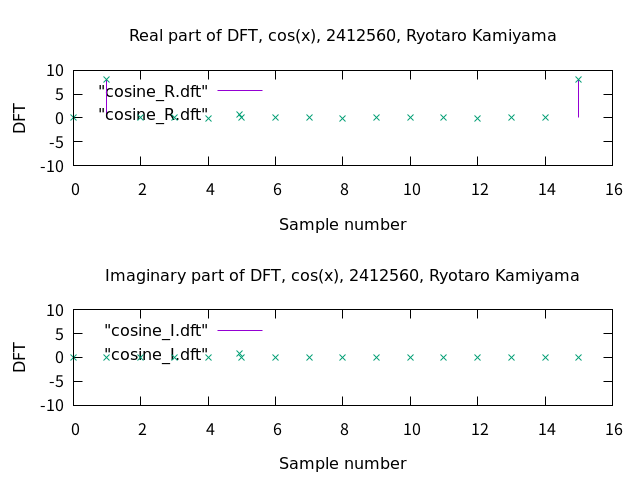
\includegraphics[width=0.7\linewidth]{cos_dft.png}
    \caption{$N=20$}
\end{figure}

また、余弦波と比較するため正弦波のDFTの結果も以下に示す。
\begin{figure}[H]
    \centering
    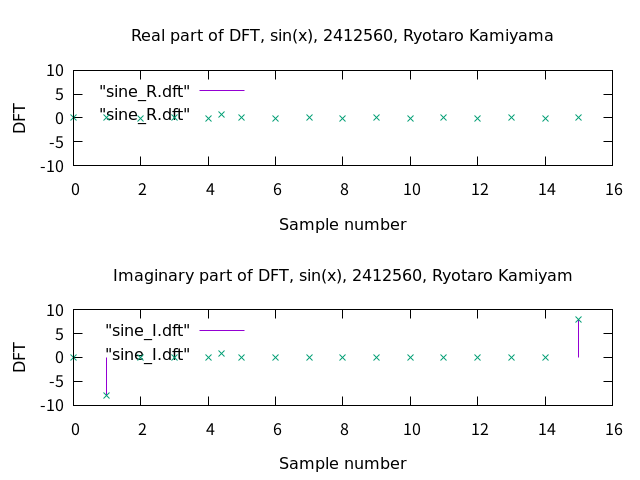
\includegraphics[width=0.7\linewidth]{sin_dft.png}
    \caption{$N=20$}
\end{figure}

余弦波では、実部の $k=1$ および $k=15$ に大きな値が現れ、
虚部はほぼ0となった。
一方、正弦波のDFTでは、
実部はほぼ0となり、
虚部の $k=1$ および $k=15$ に大きな値が現れた。
これは、
DFTの実部 $A_k$ が余弦関数との積和、
虚部 $B_k$ が正弦関数との積和によって計算されるためである。
そのため、
入力信号が余弦波の場合は実部に大きな値が現れ、
虚部はほぼ0となり、
入力信号が正弦波の場合は虚部に大きな値が現れ、
実部はほぼ0となる。


\subsection{報告事項(1-4)}
5種類の混合正弦波の DFT の結果を以下に示す。
\begin{figure}[H]
    \centering
    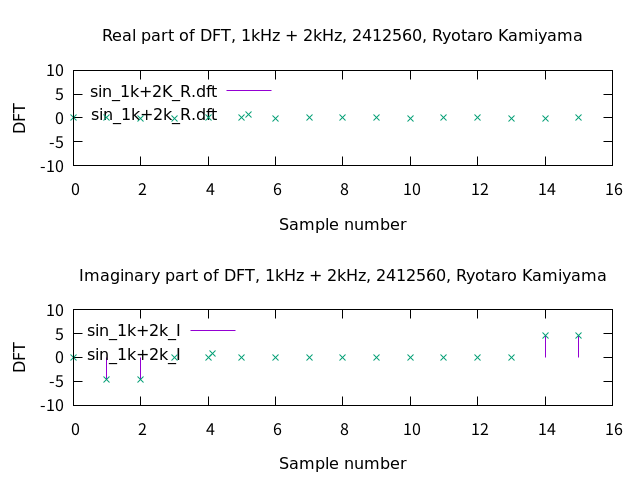
\includegraphics[width=0.7\linewidth]{mix_1k2k.png}
    \caption{$1\text{kHz}$と$2\text{kHz}$の混合波のDFT(振幅比 1:1)}
\end{figure}
\begin{figure}[H]
    \centering
    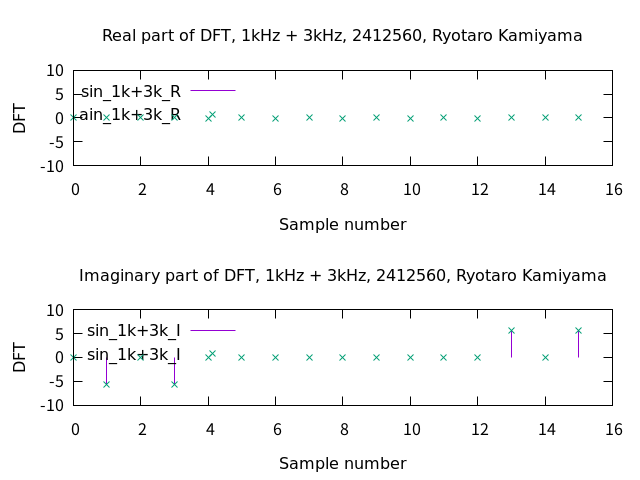
\includegraphics[width=0.7\linewidth]{mix_1k3k.png}
    \caption{$1\text{kHz}$と$3\text{kHz}$の混合波のDFT(振幅比 1:1)}
\end{figure}
\begin{figure}[H]
    \centering
    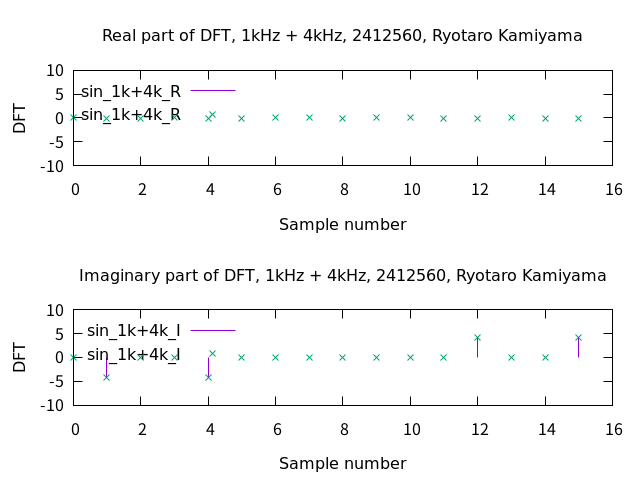
\includegraphics[width=0.7\linewidth]{mix_1k4k.png}
    \caption{$1\text{kHz}$と$4\text{kHz}$の混合波のDFT(振幅比 1:1)}
\end{figure}
\begin{figure}[H]
    \centering
    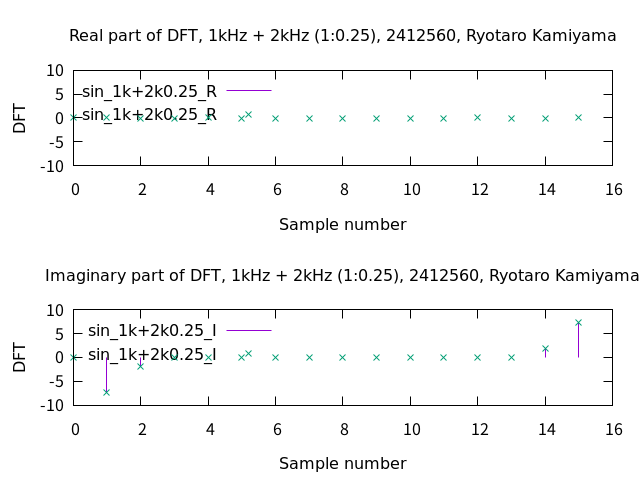
\includegraphics[width=0.7\linewidth]{mix_1k2k025.png}
    \caption{$1\text{kHz}$と$2\text{kHz}$の混合波のDFT(振幅比 1:0.25)}
\end{figure}
\begin{figure}[H]
    \centering
    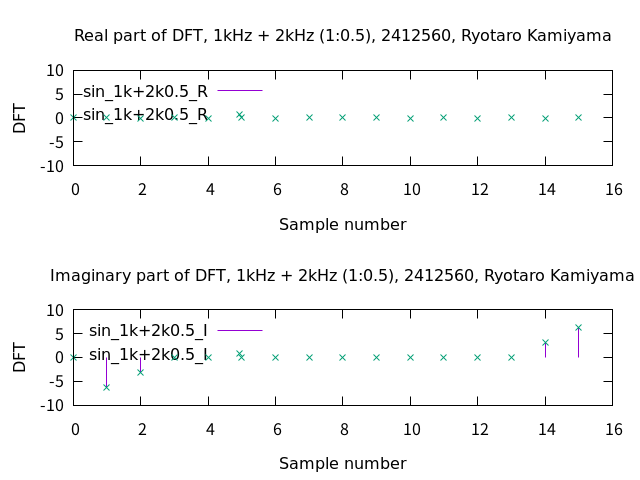
\includegraphics[width=0.7\linewidth]{mix_1k2k05.png}
    \caption{$1\text{kHz}$と$2\text{kHz}$の混合波のDFT(振幅比 1:0.5)}
\end{figure}

入力信号が正弦波であるため、
どの場合においても虚部に大きな値が現れた。
また、
振幅が等しく周波数の異なる混合波では、
それぞれの周波数に対応するサンプル番号に大きな値が現れていた。
さらに、
振幅比の異なる混合波では、
DFT結果のピーク値も入力信号の振幅比に対応して変化していた。

このことから、
DFTによって入力信号に含まれる周波数成分およびその強さを正しく抽出できていることが確認できた。

\subsection{報告事項(1-5)}
以下に未知の正弦混合波のDFTの結果を示す。
\begin{figure}[H]
    \centering
    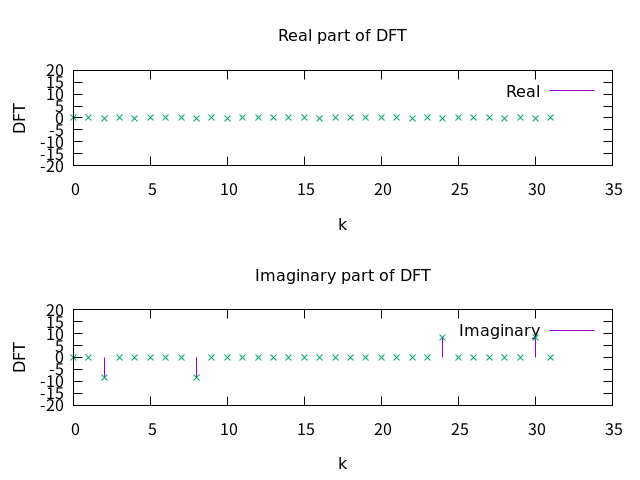
\includegraphics[width=0.7\linewidth]{sub15.png}
    \caption{未知の正弦混合波}
\end{figure}

虚部のDFT結果より、
$k=2$，$k=8$，$k=24$，$k=30$ に大きな値が現れた。
DFTでは $k$ と $N-k$ が対になって現れるため、
$k=2$ と $k=30$，
$k=8$ と $k=24$ はそれぞれ同じ周波数成分を表している。
したがって、
未知信号には $k=2$ および $k=8$ に対応する周波数成分が含まれていることが分かる。

サンプリング周波数を $f_s=16\,\mathrm{kHz}$，
DFTサイズを $N=32$ とすると、

\begin{equation}
f=\frac{k}{N}f_s
\end{equation}

より、

\begin{equation}
f_1=\frac{2}{32}\times16000
=1000\,\mathrm{Hz}
\end{equation}

\begin{equation}
f_2=\frac{8}{32}\times16000
=4000\,\mathrm{Hz}
\end{equation}

となる。
また、
$k=2$ と $k=8$ のピーク値はほぼ同じ大きさであった。

よって、
未知信号には、
$1\,\mathrm{kHz}$ と $4\,\mathrm{kHz}$ の正弦波が、
およそ $1:1$ の振幅比で含まれていると考えられる。


\subsection{報告事項(2-1)}
以下に各$N$に対するDFTの結果を示す。
\begin{figure}[H]
    \centering
    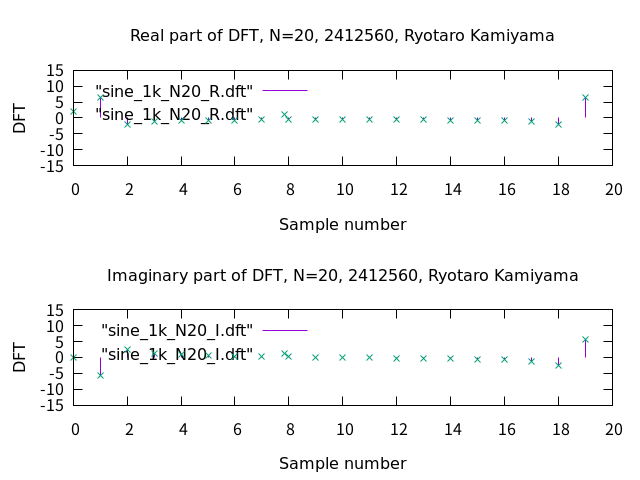
\includegraphics[width=0.7\linewidth]{sine_1k_N20.png}
    \caption{$N=20$}
\end{figure}
\begin{figure}[H]
    \centering
    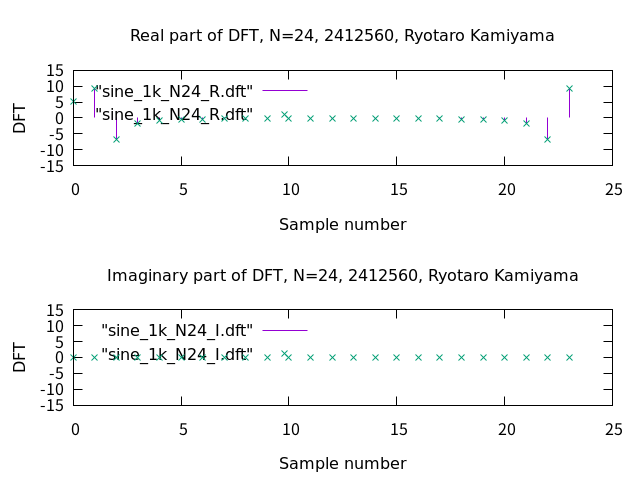
\includegraphics[width=0.7\linewidth]{sine_1k_N24.png}
    \caption{$N=24$}
\end{figure}
\begin{figure}[H]
    \centering
    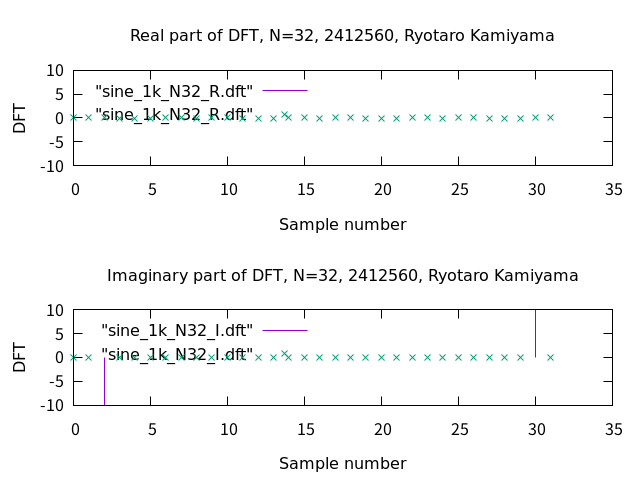
\includegraphics[width=0.7\linewidth]{sine_1k_N32.png}
    \caption{$N=32$}
\end{figure}

$N=20$ および $N=24$ の結果では、
$k=1$ 付近だけでなく、
複数のサンプル番号に成分が広がって現れた。
これは、
1\,kHz の正弦波を $N=20$ または $N=24$ で切り出した場合、
切り出した区間が信号周期の整数倍にならないためである。
DFTでは切り出した信号が周期的に繰り返されることを仮定しているため、
区間の端で不連続が生じ、
本来の周波数成分以外にも成分が現れたと考えられる。
一方、
$N=32$ の場合は、
1\,kHz の正弦波がちょうど2周期分含まれるため、
主に $k=2$ および $k=30$ に大きな値が現れた。
このため、
$N=32$ では1\,kHz の成分を比較的正しく抽出できていることが分かる。

以上より、
DFTで正しく周波数解析を行うためには、
信号周期の整数倍となる区間を切り出すことが重要である。

\subsection{報告事項(2-2)}
ハミング窓 ($N = 256$) をグラフで表示したものを以下に示す。
\begin{figure}[H]
    \centering
    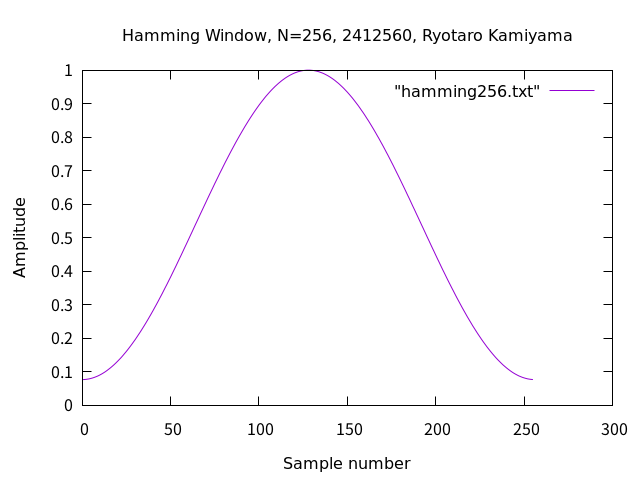
\includegraphics[width=0.7\linewidth]{hamming256.png}
    \caption{$N=256$}
\end{figure}
グラフから、中央のサンプル数128で最大になり、両端に向かって滑らかに減少する形となっていることが分かる。

\subsection{報告事項(3-1)}

"o" と "ro" の音声解析を行った。
以下にこれらの音声波形を示す。

\begin{figure}[H]
    \centering
    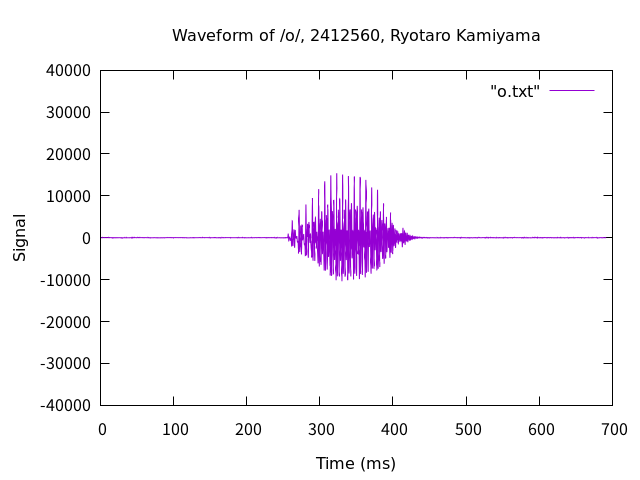
\includegraphics[width=0.7\linewidth]{o_waveform.png}
    \caption{"o" の音声波形}
\end{figure}

\begin{figure}[H]
    \centering
    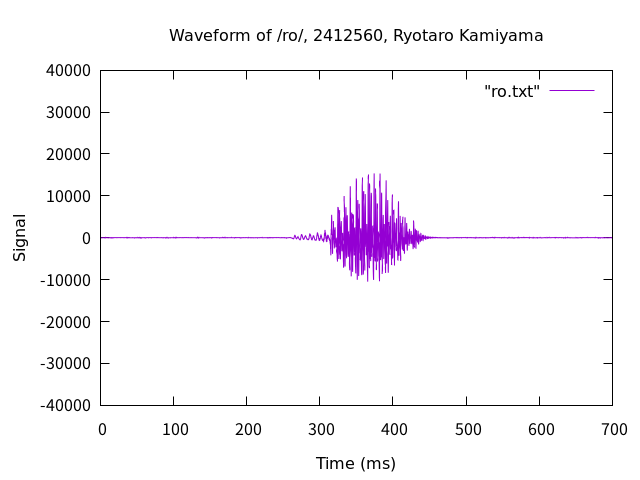
\includegraphics[width=0.7\linewidth]{ro_waveform.png}
    \caption{"ro" の音声波形}
\end{figure}

音声波形を確認した結果、
"o" の分析開始時刻は $320\,\mathrm{ms}$，
"ro" の分析開始時刻は $250\,\mathrm{ms}$ および
$320\,\mathrm{ms}$ に設定してスペクトル解析を行った。
以下にその結果を示す。

\begin{figure}[H]
    \centering
    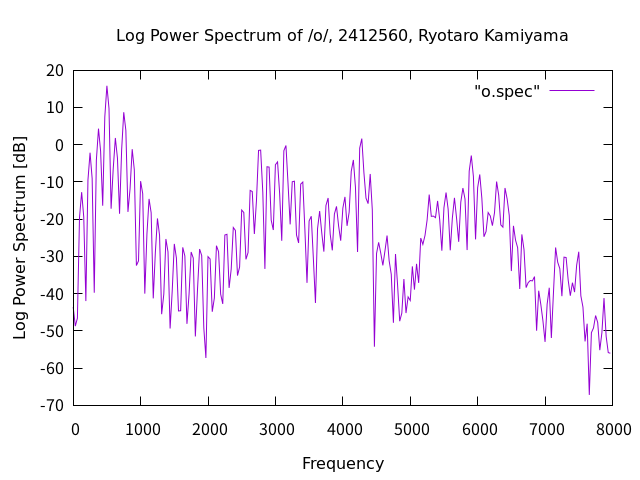
\includegraphics[width=0.7\linewidth]{o_spec.png}
    \caption{/o/ の対数パワースペクトル
    (使用音声ファイル: o.ad，
    分析開始時刻: $320\,\mathrm{ms}$，
    分析窓幅: $32\,\mathrm{ms}$)}
\end{figure}

\begin{figure}[H]
    \centering
    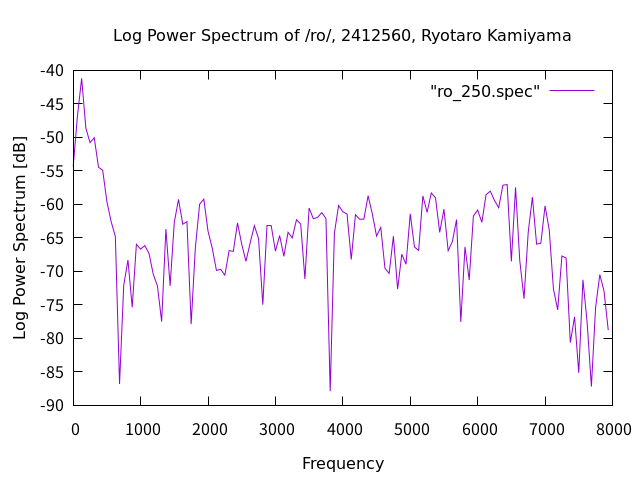
\includegraphics[width=0.7\linewidth]{ro_250_spec.png}
    \caption{/ro/ の対数パワースペクトル
    (使用音声ファイル: ro.ad，
    分析開始時刻: $250\,\mathrm{ms}$，
    分析窓幅: $32\,\mathrm{ms}$)}
\end{figure}

\begin{figure}[H]
    \centering
    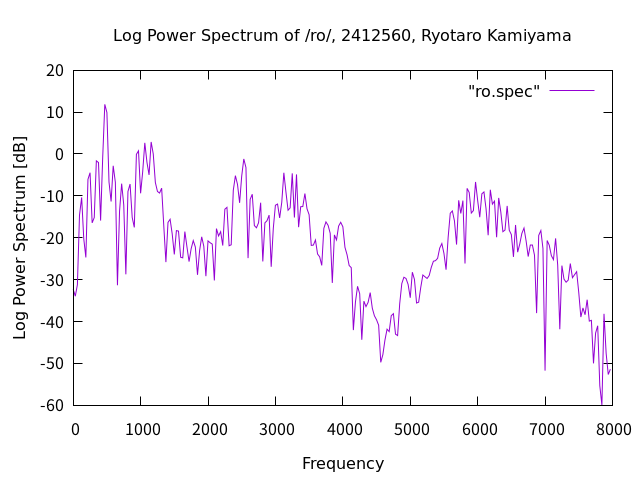
\includegraphics[width=0.7\linewidth]{ro_spec.png}
    \caption{/ro/ の対数パワースペクトル
    (使用音声ファイル: ro.ad，
    分析開始時刻: $320\,\mathrm{ms}$，
    分析窓幅: $32\,\mathrm{ms}$)}
\end{figure}

\subsection{報告事項(3-2)}
音声波形を比較すると、立ち上がりや終わりの時間は大きく変わらないが、
"ro" は子音を含んでいるため、立ち上がり部分の振幅が "o" と比べて
小さくなっていることが分かる。

また、"o" の対数パワースペクトルでは、低周波側に強いピークが確認できた。
一方、"ro" の $250\,\mathrm{ms}$ 付近では、広い周波数帯域に成分が分布していた。
これは子音 "r" を含むためであると考えられる。
さらに、"ro" の $320\,\mathrm{ms}$ 付近では、母音 "o" の成分が支配的となり、
"o" 単体の場合に近いスペクトルとなった。

このことから、母音と子音ではスペクトル特性が異なり、同じ音声でも解析する時間位置によって周波数特性が変化することが確認できた。


\subsection{報告事項(3-3)}
各音声ファイルの音声波形を以下に示す。
\begin{figure}[H]
    \centering
    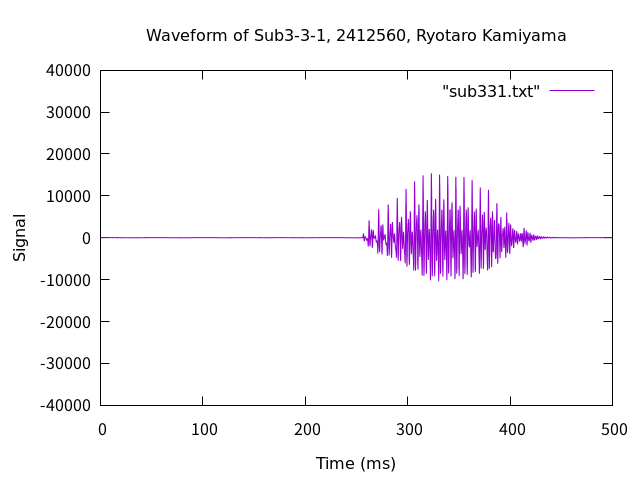
\includegraphics[width=0.7\linewidth]{sub331_wave.png}
    \caption{Sub3-3-1.adの音声波形}
\end{figure}
\begin{figure}[H]
    \centering
    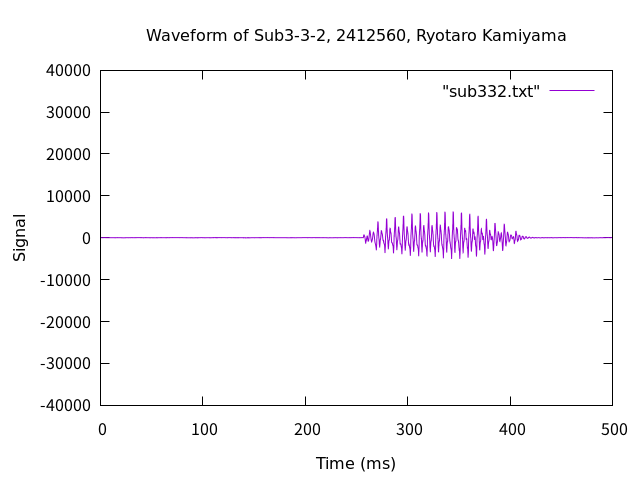
\includegraphics[width=0.7\linewidth]{sub332_wave.png}
    \caption{Sub3-3-2.adの音声波形}
\end{figure}
\begin{figure}[H]
    \centering
    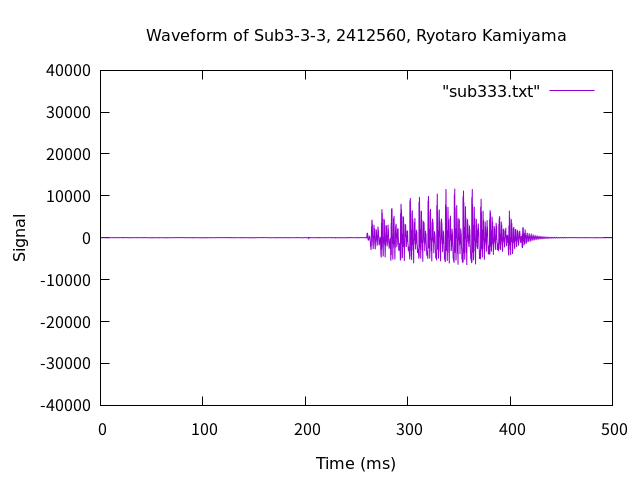
\includegraphics[width=0.7\linewidth]{sub333_wave.png}
    \caption{Sub3-3-3.adの音声波形}
\end{figure}


これらの音声波形から分析開始時刻をすべて$320\,\mathrm{ms}$と設定し、スペクトル解析を行った。
以下にその結果を示す。
\begin{figure}[H]
    \centering
    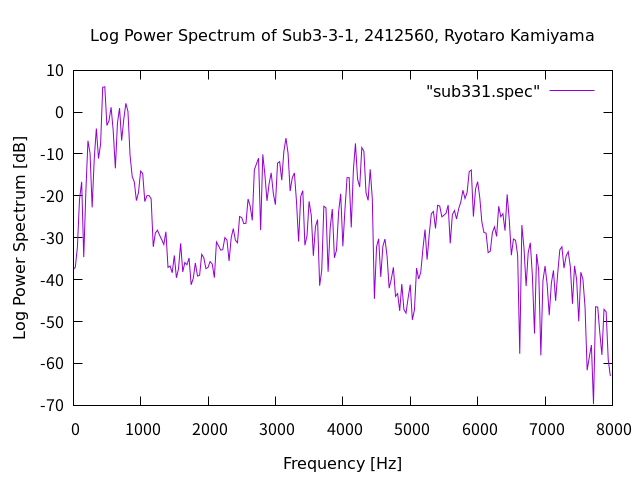
\includegraphics[width=0.7\linewidth]{sub331_spec.png}
    \caption{Sub3-3-1.adの音声スペクトル}
\end{figure}
\begin{figure}[H]
    \centering
    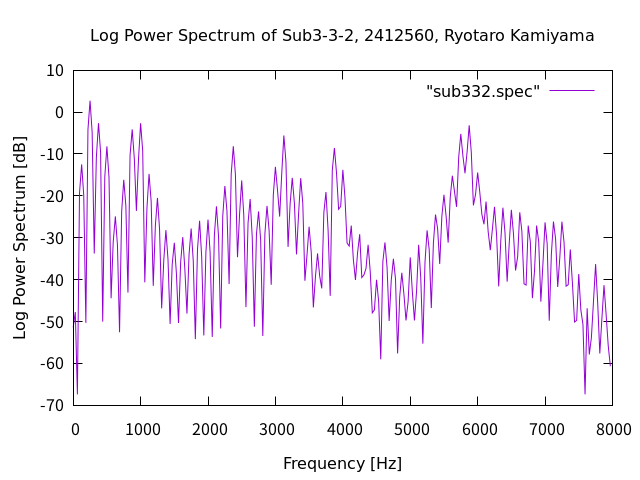
\includegraphics[width=0.7\linewidth]{sub332_spec.png}
    \caption{Sub3-3-2.adの音声スペクトル}
\end{figure}
\begin{figure}[H]
    \centering
    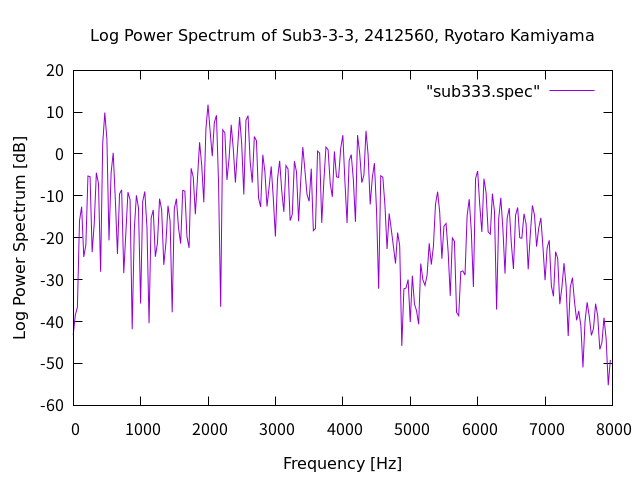
\includegraphics[width=0.7\linewidth]{sub333_spec.png}
    \caption{Sub3-3-3.adの音声スペクトル}
\end{figure}

つぎにこれらの対数パワースペクトルから、スペクトル包絡をフリーハンドで求めた。
以下にスペクトル包絡を書き込んだ図を示す。

\begin{figure}[H]
    \centering
    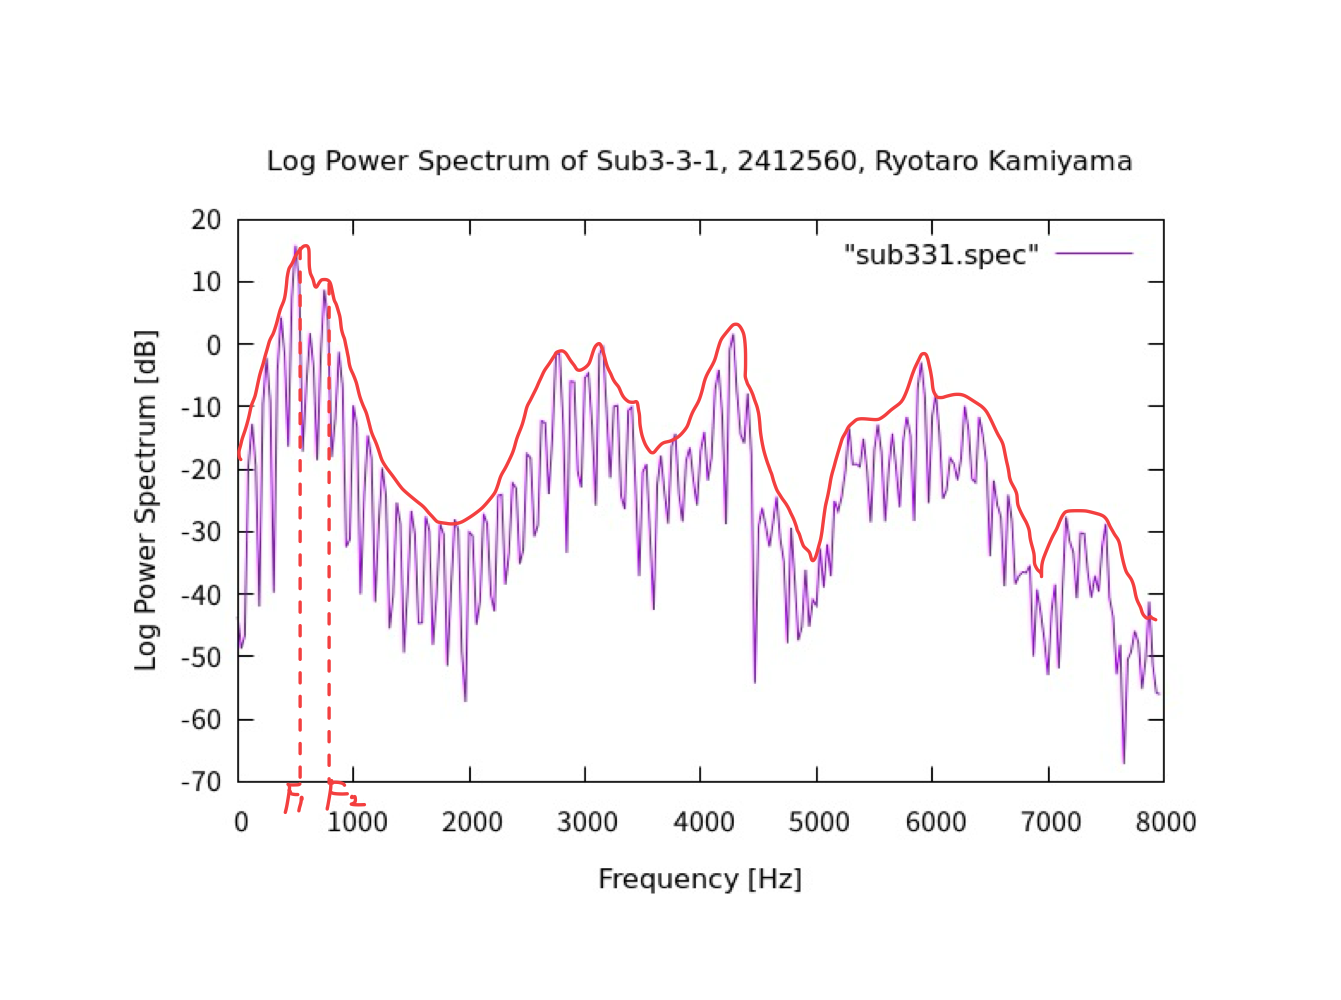
\includegraphics[width=0.8\linewidth]{000.png}
    \caption{Sub3-3-1.adのスペクトル包絡}
\end{figure}
\begin{figure}[H]
    \centering
    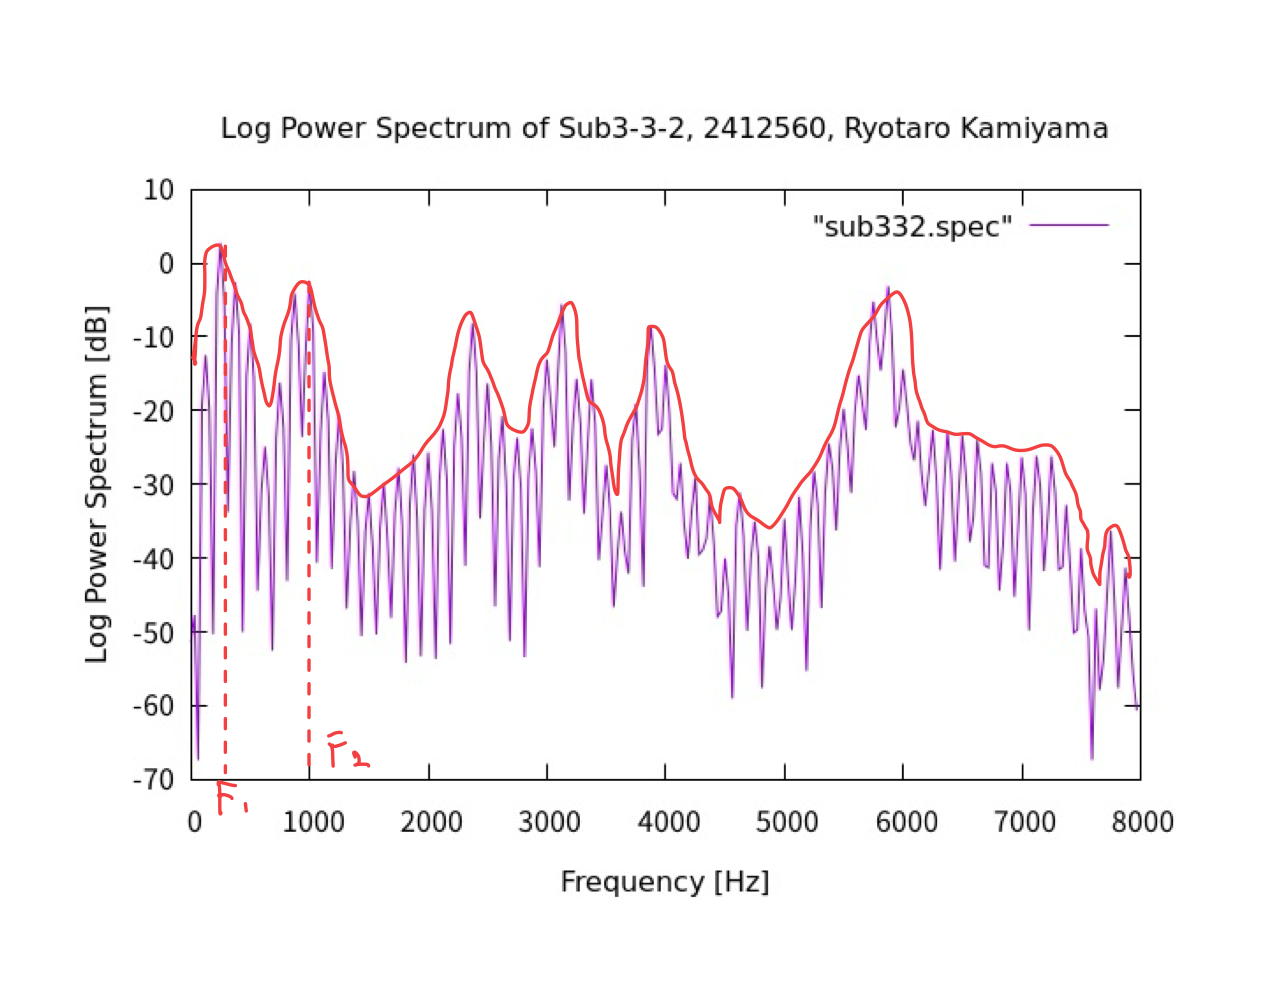
\includegraphics[width=0.7\linewidth]{001.png}
    \caption{Sub3-3-2.adのスペクトル包絡}
\end{figure}
\begin{figure}[H]
    \centering
    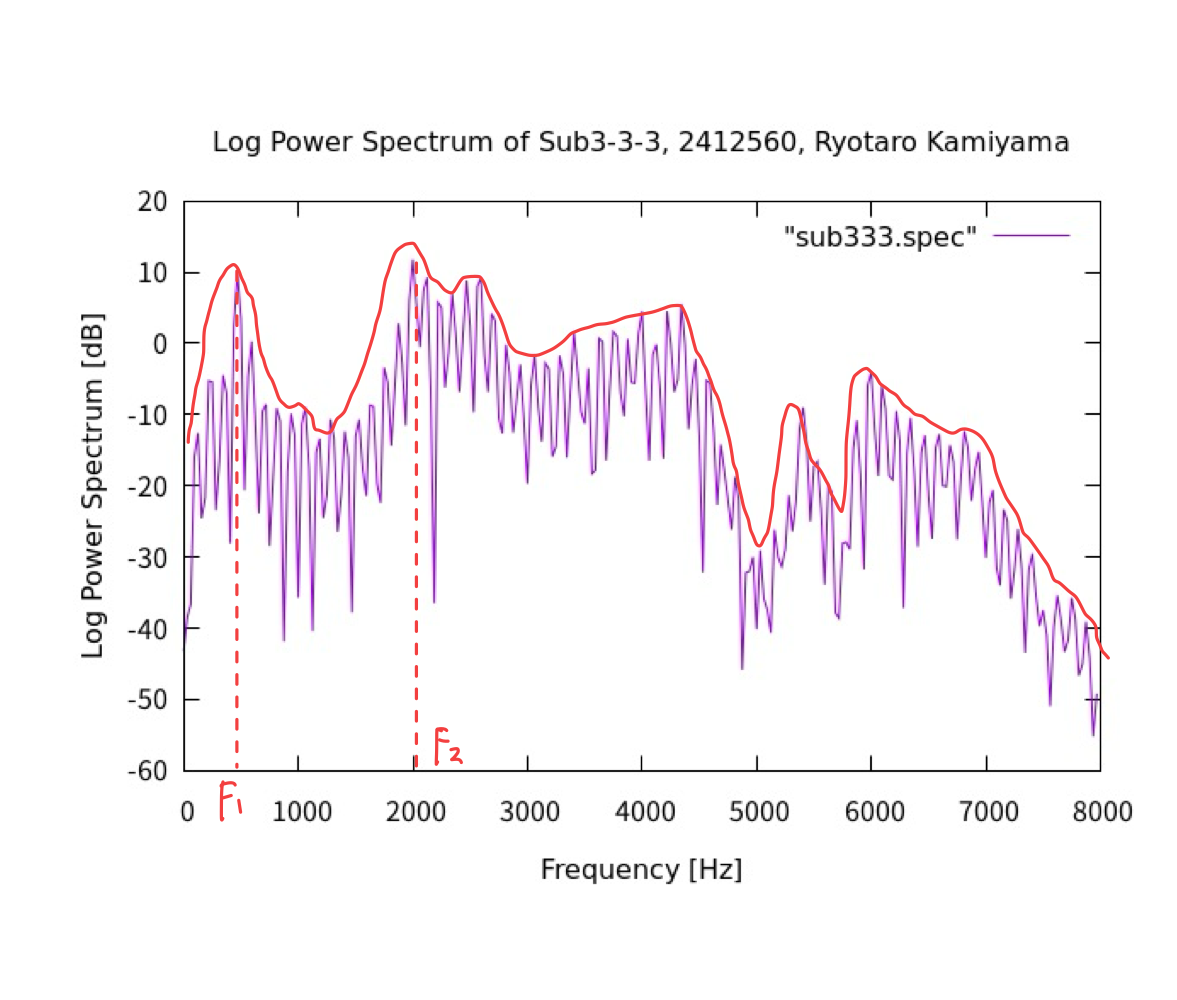
\includegraphics[width=0.7\linewidth]{002.png}
    \caption{Sub3-3-3.adのスペクトル包絡}
\end{figure}
これらのスペクトル包絡から第１フォルマント周波数と第２フォルマント周波数を読み取った結果を以下にまとめた。
\begin{table}[H]
    \centering
    \caption{未知音声データのフォルマント周波数}
    \begin{tabular}{c c c}
        \hline
        音声データ & $F_1$ [Hz] & $F_2$ [Hz] \\
        \hline
        Sub3-3-1 & 500 & 800 \\
        Sub3-3-2 & 300 & 1000 \\
        Sub3-3-3 & 450 & 2000 \\
        \hline
    \end{tabular}
\end{table}
得られたフォルマント周波数対 (F1, F2) を、日本語 5 母音 (a, e, i, o, u) の典型的なフォ
ルマント分布 とともに図示した。
\begin{figure}[H]
    \centering
    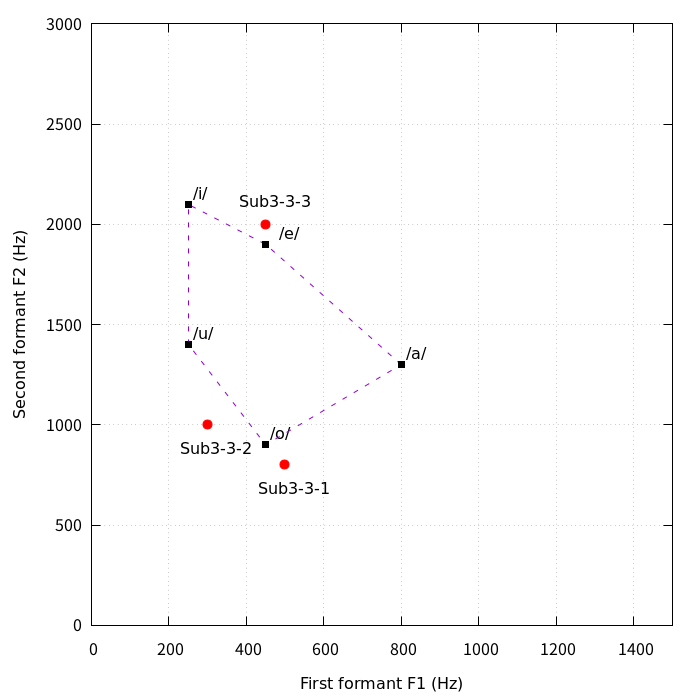
\includegraphics[width=0.7\linewidth]{formant2.png}
    \caption{フォルマント分布}
\end{figure}
Sub3-3-1 は、
/o/ の位置に最も近い場所に存在している。
そのため、
Sub3-3-1 は母音 /o/ であると推定した。

Sub3-3-2 は、
/u/ と/o/に比較的近い位置に存在している。Sub3-3-1の方が/o/と近い距離にあるため、
Sub3-3-2 は母音 /u/ であると推定した。

Sub3-3-3 は、
/e/ および /i/ に近い位置に存在しているが、
特に /e/ の位置に近いことから、
Sub3-3-3 は母音 /e/ であると推定した。

\section{宿題}
\subsection*{(WH1)}

ナイキスト周波数とは、
サンプリング周波数 $f_s$ の半分の周波数であり、

\begin{equation}
f_N=\frac{f_s}{2}
\end{equation}

で表される。
今回の実験では、
サンプリング周波数は $16\,\mathrm{kHz}$ であったため、

\begin{equation}
f_N=\frac{16000}{2}=8000\,\mathrm{Hz}
\end{equation}

となる。
実際に、
対数パワースペクトルの周波数範囲は
$0\sim8000\,\mathrm{Hz}$ で表示されていた。
ナイキスト周波数を超える周波数成分を含む信号をサンプリングすると、
折り返し雑音（エイリアシング）が発生し、
本来とは異なる周波数成分として観測される。
そのため、
音声信号を正しく解析するためには、
ナイキスト周波数以下の周波数成分のみを扱うことが重要である。
\subsection*{(WH2)}

DFTは

\begin{equation}
X_k=
\sum_{n=0}^{N-1}
x_n e^{-j\frac{2\pi nk}{N}}
\end{equation}

で定義される。
ここで、
$k$ を $N-k$ に置き換えると、

\begin{align}
X_{N-k}
&=
\sum_{n=0}^{N-1}
x_n
e^{-j\frac{2\pi n(N-k)}{N}} \\
&=
\sum_{n=0}^{N-1}
x_n
e^{-j2\pi n}
e^{j\frac{2\pi nk}{N}}
\end{align}

となる。
$n$ は整数であるため、

\begin{equation}
e^{-j2\pi n}=1
\end{equation}

である。
したがって、

\begin{equation}
X_{N-k}
=
\sum_{n=0}^{N-1}
x_n
e^{j\frac{2\pi nk}{N}}
\end{equation}

となる。
一方、

\begin{equation}
X_{-k}
=
\sum_{n=0}^{N-1}
x_n
e^{-j\frac{2\pi n(-k)}{N}}
=
\sum_{n=0}^{N-1}
x_n
e^{j\frac{2\pi nk}{N}}
\end{equation}

である。
よって、

\begin{equation}
X_{N-k}=X_{-k}
\end{equation}

が成り立つ。

\subsection*{(WH3)}
窓関数には、
ハミング窓のほかに、
ハン窓、
ブラックマン窓、
ブラックマンハリス窓などが存在する。

ハン窓は，

\begin{equation}
w_n
=
\frac{1}{2}
\left(
1-\cos\frac{2\pi n}{N}
\right)
\end{equation}

で表される。
サイドローブ成分を小さくできるため、
スペクトル漏れを抑えやすい特徴を持つ。

ブラックマン窓は、

\begin{equation}
w_n
=
0.42
-
0.5\cos\frac{2\pi n}{N}
+
0.08\cos\frac{4\pi n}{N}
\end{equation}

で表される。
ハン窓よりもさらにサイドローブ成分を小さく抑えられる特徴を持つ。
一方で、
メインローブ幅が広くなるため、
周波数分解能は低下する。

ブラックマンハリス窓は、

\begin{equation}
w_n
=
0.42
-
0.48829\cos\frac{2\pi n}{N}
+
0.14128\cos\frac{4\pi n}{N}
-
0.01168\cos\frac{6\pi n}{N}
\end{equation}

で表される。
ブラックマン窓よりもさらにサイドローブ成分を小さく抑えられる窓関数であり、
不要な周波数成分の影響をより小さくできる特徴を持つ。

\subsection*{(WH4)}
フォルマントとは、
音声スペクトルにおいて特に強く現れる周波数成分のことである。
声は声帯で作られた音が声道を通ることで作られ、
声道の共鳴によって特定の周波数成分が強められる。
この強められた周波数成分がフォルマントである。
フォルマントは周波数の低い順に
第1フォルマント $F_1$，
第2フォルマント $F_2$
と呼ばれる。
一般に、
$F_1$ は口の開き具合、
$F_2$ は舌の前後位置と関係しており、
母音ごとに異なるフォルマント周波数対 $(F_1,F_2)$ を持つ。

今回の実験では、
未知音声データから求めたフォルマント周波数対 $(F_1,F_2)$ を用いることで、
母音を推定することができた。
\section{結論}
DFT、
窓関数、
スペクトル解析を用いた音声解析を行った。
その結果、
入力信号に含まれる周波数成分やフォルマント周波数を求めることができ、
周波数解析や母音識別の基本的な仕組みについて理解することができた。
\section{感想}
スペクトル包絡やフォルマント分布を用いることで、
音声の特徴を視覚的に確認できることが分かり、
音声信号処理の面白さを感じた。
また、
録音音声の文字起こしなどで、
どのように音声を判別しているのかという基本的な仕組みを理解することができた。
\section{参考文献}

\begin{thebibliography}{99}

\bibitem{ref1}
「ナイキスト周波数とは？信号処理におけるサンプリングレートの基礎」,
\url{https://words.af-e.net/nyquist-frequency/},
（参照 2026-05-27）.

\bibitem{ref2}
瓜田 陽一郎,
「FFTの窓関数比較」,
\url{https://rm-engineering.info/fft-window-function-comparison/#i-7},
（参照 2026-05-27）.

\bibitem{ref3}
kennzo,
「窓関数」,
\url{https://www.kennzo.net/window-function},
（参照 2026-05-27）.

\bibitem{ref4}
「フォルマントとは？音声の『個性』を決める音の指紋を徹底解説」,
\url{https://omomuki-tech.com/archives/6274},
（参照 2026-05-27）.
\end{thebibliography}

\end{document}